% This file was created with tikzplotlib v0.10.1.
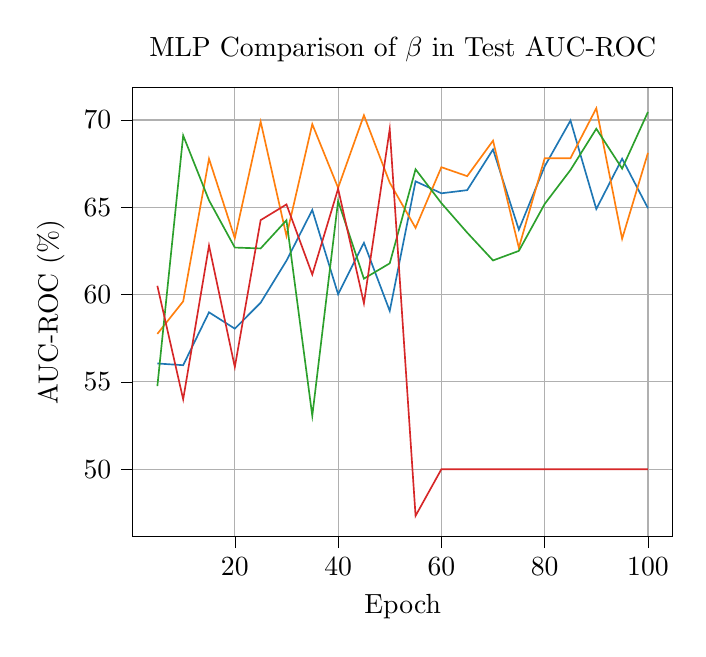
\begin{tikzpicture}

\definecolor{crimson2143940}{RGB}{214,39,40}
\definecolor{darkgray176}{RGB}{176,176,176}
\definecolor{darkorange25512714}{RGB}{255,127,14}
\definecolor{forestgreen4416044}{RGB}{44,160,44}
\definecolor{steelblue31119180}{RGB}{31,119,180}

\begin{axis}[
tick align=outside,
tick pos=left,
title={MLP Comparison of $\beta$ in Test AUC-ROC},
x grid style={darkgray176},
xlabel={Epoch},
xmajorgrids,
xmin=0.25, xmax=104.75,
xtick style={color=black},
y grid style={darkgray176},
ylabel={AUC-ROC (\%)},
ymajorgrids,
ymin=46.1652843818146, ymax=71.8430438527479,
ytick style={color=black}
]
\addplot [semithick, steelblue31119180]
table {%
5 56.0574004597166
10 55.9587938494108
15 58.988233949415
20 58.0517054703633
25 59.5378178797582
30 61.9442093264535
35 64.8498874415715
40 60.0235295280347
45 62.971660653213
50 59.0657351644687
55 66.4906219516673
60 65.804365853233
65 65.9855391958372
70 68.3149295474348
75 63.72268502442
80 67.3458992940887
85 69.9721620077673
90 64.9032032052118
95 67.7872733540057
100 64.9516550326765
};
\addplot [semithick, darkorange25512714]
table {%
5 57.752109782597
10 59.614922986193
15 67.7821420741404
20 63.2335690347065
25 69.9079348940483
30 63.36081681402
35 69.76374026764
40 66.1180334074001
45 70.2719011920898
50 66.4131188640023
55 63.8221495336682
60 67.2995939741557
65 66.7869285301775
70 68.819200730295
75 62.6884875498075
80 67.8092955226281
85 67.8159821763673
90 70.6758729677055
95 63.1978676764659
100 68.1180622949796
};
\addplot [semithick, forestgreen4416044]
table {%
5 54.758478175183
10 69.1151562992072
15 65.4014700092719
20 62.6968421383493
25 62.6468775869635
30 64.2610516926704
35 53.0599866046144
40 65.365739195474
45 60.9144146180524
50 61.7936055738023
55 67.1785382608249
60 65.2419543114951
65 63.5505034633982
70 61.9586411258466
75 62.5051876206583
80 65.1925434402597
85 67.1415092577701
90 69.5024756452378
95 67.2204026041308
100 70.458224596203
};
\addplot [semithick, crimson2143940]
table {%
5 60.5050824510686
10 54.0061905991575
15 62.8102434538045
20 55.8534352040543
25 64.2677566516616
30 65.1676569500176
35 61.1516405658093
40 66.0646684334822
45 59.5051274164633
50 69.4863134267092
55 47.332455266857
60 50
65 50
70 50
75 50
80 50
85 50
90 50
95 50
100 50
};
\end{axis}

\end{tikzpicture}
